% house_prelim.tex: HOUSE COPY of definite_integrals/common/prelim_style.tex; [HOUSE] titles from \housechapter
% =====================================================================
% prelim_style.tex: makes the Test look like a Singapore JC H2 Mathematics
% 9758 prelim paper (studied from ACJC/RI 2026 P1/P2 on the box:
% body Times New Roman + Times-style maths, cover in Arial).
% Fonts: prelim_fonts.tex (real Times New Roman/Arial + Times-style maths).
% Shared by Ch10 (di_style) and Ch11 (de_style; sets \prelimtitle/\prelimsubject). Loaded AFTER the chapter style (overrides its layout for the test only).
% =====================================================================
% [HOUSE] fonts loaded by house.tex
\providecommand{\prelimtitle}{\MakeUppercase{\housechap} TEST}
\providecommand{\prelimsubject}{\housechap}
\geometry{a4paper, top=22mm, bottom=24mm, left=25mm, right=25mm, headsep=6mm, footskip=12mm}
\setlength{\parindent}{0pt}
\setlength{\parskip}{0.9ex plus 0.3ex minus 0.2ex}
\linespread{1.3}
\setlength{\emergencystretch}{3em}
\clubpenalty=10000 \widowpenalty=10000 \interlinepenalty=10000
\AtBeginDocument{\fontsize{12}{14.4}\selectfont}
\renewcommand{\normalsize}{\fontsize{12}{14.4}\selectfont}

% ---- figures: plain black/grey like a printed paper ----------------------
\ifdefined\prelimkeepcolour\else % question paper: black/grey figures; solutions keep colour
\pgfplotsset{curve/.style={black, semithick, smooth, samples=150},
  line2/.style={black, semithick, samples=2},
  sketch/.append style={axis line style={thin, black}, every axis label/.append style={black}}}
\tikzset{region/.style={fill=black!15, draw=none}, regionB/.style={fill=black!30, draw=none},
  rect/.style={fill=black!8, draw=black, thin}, ax3/.style={-{Stealth[length=1.5mm]}, thin, black}}
\colorlet{blue}{black}\colorlet{red}{black}\colorlet{orange}{black}
\fi

% ---- header / footer: page number centred top (bold), [Turn over at bottom right
\makeatletter
\providecommand{\prelimfootlabel}{\prelimtitle\ 2026}
\newcommand{\pp@footer}{{\coverfont\scriptsize \prelimfootlabel\hspace{3em}H2 MATHEMATICS 9758}}
\fancypagestyle{prelim}{\fancyhf{}%
  \chead{\bfseries\thepage}%
  \lfoot{\pp@footer}%
  \rfoot{\ifnum\value{page}<\getpagerefnumber{LastPage}\relax\textbf{[Turn over}\fi}%
  \renewcommand{\headrulewidth}{0pt}\renewcommand{\footrulewidth}{0pt}}
\fancypagestyle{prelimcover}{\fancyhf{}%
  \rfoot{\coverfont\textbf{[Turn over}}%
  \renewcommand{\headrulewidth}{0pt}\renewcommand{\footrulewidth}{0pt}}
\pagestyle{prelim}

% ---- marks: [n] regular weight, right-aligned at the end of the part ----------
\renewcommand{\mk}[1]{{\unskip\nobreak\hfil\penalty50\hskip1.5em\hbox{}\nobreak\hfill[#1]%
  \parfillskip=0pt\finalhyphendemerits=0\par}}

% ---- questions: bold number at the left margin, text indented; grey [tag] straight after the number (3B)
\newsavebox{\pp@qmeas}
\newcommand{\pp@qlist}[1]{%
  \begin{list}{}{\setlength\leftmargin{2.6em}\setlength\labelwidth{2.1em}\setlength\labelsep{0.5em}%
     \setlength\topsep{0pt}\setlength\itemsep{0pt}\setlength\parsep{0.9ex}%
     \renewcommand\makelabel[1]{\textbf{##1}\hfil}}%
  \item[\thediq]\@endparpenalty\@M\setbox0=\hbox{\di@tag{#1}}\ifdim\wd0=0pt\else{\small\textcolor{black!60}{[\di@tag{#1}]}}\par\nobreak\fi\csname diQbody@#1\endcsname\par\penalty\@M
  \end{list}}
% a question starts on a new page unless it fits whole on the current one
% (questions taller than a page may break, but only between parts)
\renewcommand{\putQ}[1]{\stepcounter{diq}%
  \expandafter\xdef\csname diLab@#1\endcsname{\thediq}%
  \par\setbox\pp@qmeas=\vbox{\pp@qlist{#1}}%
  \ifdim\dimexpr\ht\pp@qmeas+\dp\pp@qmeas\relax<0.95\textheight
    \needspace{\dimexpr\ht\pp@qmeas+\dp\pp@qmeas\relax}\else\needspace{14\baselineskip}\fi
  \zsavepos{q-s\thediq}\pp@qlist{#1}\par\zsavepos{q-e\thediq}\vspace{5ex plus 2ex minus 1ex}}
% part labels (a)/(i) bold, indented under the question text
\renewenvironment{qparts}[1][2.6em]{\begin{list}{}{\setlength\leftmargin{#1}%
  \setlength\labelwidth{\dimexpr#1-0.5em\relax}\setlength\labelsep{0.5em}%
  \setlength\itemsep{1.4ex}\setlength\topsep{1.2ex}\setlength\parsep{0.8ex}%
  \renewcommand\makelabel[1]{\textbf{##1}\hfil}}}{\end{list}}
\makeatother

% ---- cover page --------------------------------------------------------------
% A-level H2 style cover (9 Nov 2026; reference house_format/ref/alevel_cover_ref.png), no logos/barcodes.
% \prelimcover{total marks}{duration}{date}; heading block from \housechap; override with
% \prelimcoverhead (4 lines) and \prelimcoverline (the line under MATHEMATICS).
\makeatletter
\providecommand{\prelimcoverhead}{MAXIMUS PUNG JUN\\ H2 Mathematics (9758)\\ \housechap\\ Chapter Test}
\providecommand{\prelimcoverline}{\prelimsubject\ Test}
\newcommand{\pp@htwo}{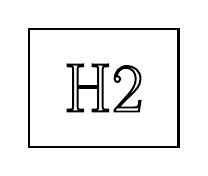
\begin{tikzpicture}[baseline=(b.base)]
  \node[draw, line width=0.9pt, minimum width=19mm, minimum height=15mm, inner sep=0pt] (b)
    {\fontsize{38}{38}\selectfont\special{pdf:literal direct 1 Tr 0.7 w}H2\special{pdf:literal direct 0 Tr}};
  \end{tikzpicture}}
\newcommand{\prelimcover}[3]{% #1 total marks, #2 duration, #3 date line
\thispagestyle{prelimcover}%
{\coverfont\fontsize{11}{13.5}\selectfont\linespread{1}\selectfont\setlength{\parskip}{0pt}%
\vspace*{4mm}
\noindent\begin{tabular}{@{}l@{\hspace{5mm}}l@{}}\raisebox{-0.5\height}{\pp@htwo}&
  \raisebox{-0.5\height}{\begin{minipage}{120mm}\fontsize{12}{14.5}\selectfont\prelimcoverhead\end{minipage}}\end{tabular}\par
\vspace{9mm}
\noindent\rule{\linewidth}{0.8pt}\par\vspace{1.2mm}
\noindent{\fontsize{12}{14.5}\selectfont\bfseries MATHEMATICS\hfill 9758}\par\vspace{1.2mm}
\noindent\prelimcoverline\hfill\textbf{#3}\par\vspace{1.2mm}
\setbox0=\hbox{#2}\ifdim\wd0>0pt \noindent\hfill\textbf{#2}\par\fi
\vspace{3mm}
\noindent You must answer on writing paper.\par\vspace{3mm}
\noindent\begin{tabular}{@{}l@{\hspace{2mm}}l@{}}You will need:&Writing paper\\ &List of formulae and results (MF27)\end{tabular}\par
\vspace{2mm}
\noindent\rule{\linewidth}{0.8pt}\par\vspace{1.5mm}
\noindent{\bfseries INSTRUCTIONS}\par\vspace{0.5mm}
\begin{list}{\textbullet}{\setlength\leftmargin{7mm}\setlength\labelwidth{4mm}\setlength\labelsep{3mm}\setlength\itemsep{0.6mm}\setlength\topsep{0pt}\setlength\parsep{0pt}}
\item Answer \textbf{all} questions.
\item Give non-exact numerical answers correct to 3 significant figures, or 1 decimal place for angles in degrees, unless a different level of accuracy is specified in the question.
\item You should use an approved graphing calculator.
\item Unsupported answers from a graphing calculator are allowed unless a question specifically states otherwise.
\item Where unsupported answers from a graphing calculator are \textbf{not} allowed in a question, you must present the mathematical steps using mathematical notations and not calculator commands.
\item You must show all working clearly.
\end{list}
\vspace{6mm}
\noindent{\bfseries INFORMATION}\par\vspace{0.5mm}
\begin{list}{\textbullet}{\setlength\leftmargin{7mm}\setlength\labelwidth{4mm}\setlength\labelsep{3mm}\setlength\itemsep{0.6mm}\setlength\topsep{0pt}\setlength\parsep{0pt}}
\item The total mark for this paper is #1.
\item The number of marks for each question or part question is shown in brackets [\ ].
\end{list}
\vfill
\noindent\rule{\linewidth}{0.8pt}\par\vspace{1mm}
\centerline{This document has \textbf{\pageref{LastPage}} pages.}\par\vspace{2mm}
}\clearpage}
\makeatother

% ---- solutions header block (page 1 of the worked solutions; same cover style) ----
\newcommand{\prelimsolhead}[1]{% #1 total marks
{\coverfont\fontsize{10}{12}\selectfont\linespread{1}\selectfont
\noindent{\bfseries \prelimtitle}\\[0.2ex]{\bfseries Compiled by Maximus Pung Jun}\\[1.6ex]Higher 2\par\vspace{2ex}
\noindent\rule{\linewidth}{1.2pt}\par\vspace{0.4ex}
\noindent{\Large\bfseries MATHEMATICS}\hfill{\Large\bfseries 9758}\par\vspace{1.2ex}
\noindent \prelimsubject\hfill\textbf{2026}\\
WORKED SOLUTIONS\hfill\textbf{Total marks: #1}\par\vspace{1ex}
\noindent\rule{\linewidth}{0.6pt}\par}\vspace{4ex}}
